\chapter{Livello di rete}
\section{Overview del libeello di rete}
\dfn{Livello di rete}{
    Il \textbf{livello di rete} (Network Layer) è responsabile del trasporto dei pacchetti da un host mittente a un host destinatario attraverso una o più reti intermedie, collandosi sopra il Data Link Layer e sotto il livello di trasporto
}

GLi obbiettivi princiapali del Network Layer sono:
\begin{itemize}
    \item \textbf{Modello di servizio}: definisce come il livello di rete fornisce il servizio ai livelli superiori
    \item \textbf{Instradamento e forwarding}:
    \begin{itemize}
        \item \textbf{Forwarding}: trasmissione di un pacchetto dall’ingresso di un router alla sua uscita appropriata.
        \item \textbf{Routing}: determinazione del percorso che i pacchetti devono seguire attraverso la rete.
    \end{itemize}
\end{itemize}

\subsection{Fuznioni del network layer}
Il Network Layer può essere suddiviso in due funzioni principali:
\begin{itemize}
    \item \textbf{Data Plane}: gestione del traffico dei pacchetti in tempo reale (forwarding)
    \item \textbf{Control Plane} (piano di controllo): determinazione del percorso ottimale per i pacchetti (routing)
\end{itemize}

Adesso vediamo entrambi nel dettaglio:

\subsubsection{Data Plane}
Il Data Plane è la parte del Network Layer responsabile della gestione effettiva del traffico dei pacchetti in tempo reale. A differenza del Control Plane, che decide il percorso dei pacchetti, il Data Plane si occupa di spostarli da un router all’altro fino alla destinazione.

Esistono due principali approcci alla gestione del Control Plane:

\begin{itemize}
    \item \textbf{Per-Router Control Plane}: ogni ruoter ha il proprio algoritmo di routing e prende decisioni autonomamente e comunicano tra di loro per scambiarsi informazioni di instradamento
    \begin{center}
        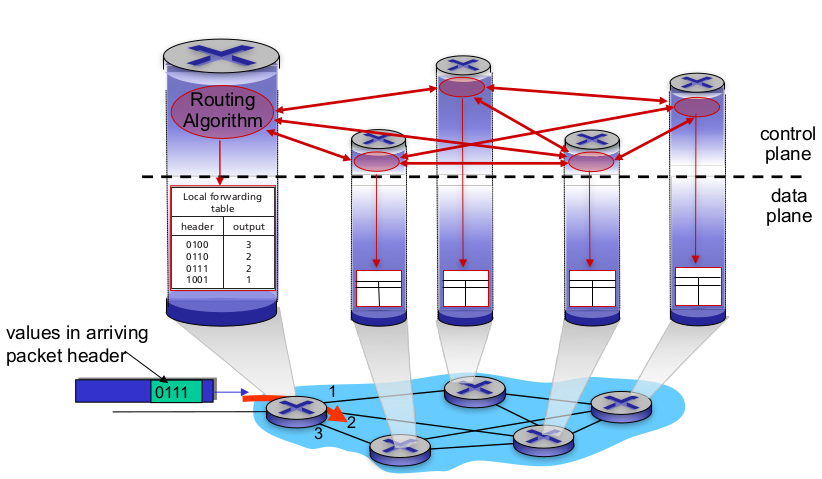
\includegraphics[width=10cm]{img/pre-router_control_plane.png}
    \end{center}
    \item \textbf{Logically Centralized Control Plane}: Un controller centralizzato (tipicamente remoto) prende le decisioni di instradamento e le comunica ai router, i router eseguono solo il forwarding senza prendere decisioni di routing
    \begin{center}
        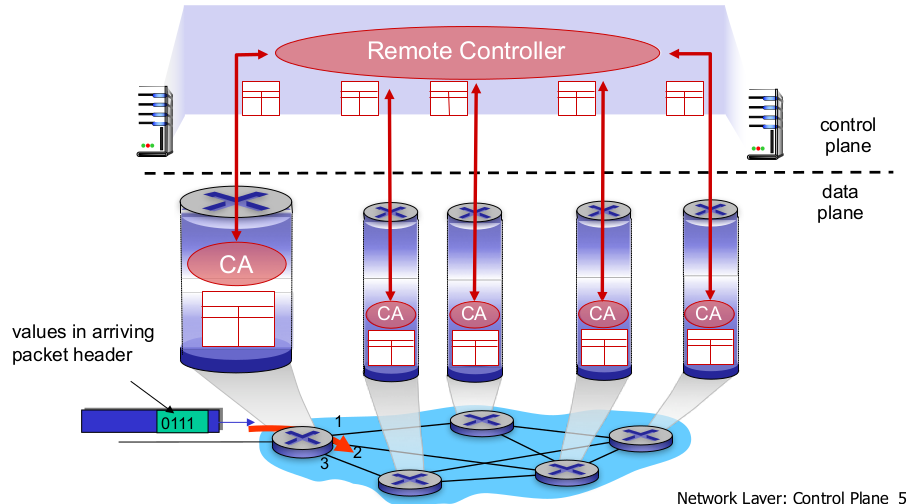
\includegraphics[width=10cm]{img/centralized_control_plane.png}
    \end{center}
\end{itemize}

In quasi tutte le infrastrutture di rete viene utilizzata il Logically Centralized Control Plane, mentre il Per-Router Control Plane viene utilizzata sopratutto nei sistemi di rete dinamici (ad esempio bluetooth col cellulare e altri dispositivi)

Fare le altre robe

\section{Router}
